%!TEX root = ../dissertation.tex
\begin{savequote}[75mm]
Knowledge knows no bounds.
\qauthor{Creator}
\end{savequote}

\chapter{Motivation and Theory}
%\newthought{There's something out there that we don't know.} 

%%%%%%%%%%%%%%%%
\section{The Standard Model and the Higgs Boson}
\paragraph{}
The Standard Model(SM) ~\cite{Pdg,Griffiths,Tully,Schwartz} is a quantum field theory describing the fundamental particles, shown in Figure~\ref{fig:SM}. So far, the SM predictions agree extremely well with experimental observations.

\begin{figure}[h!]
  \centering
  \captionsetup{justification=centering}
  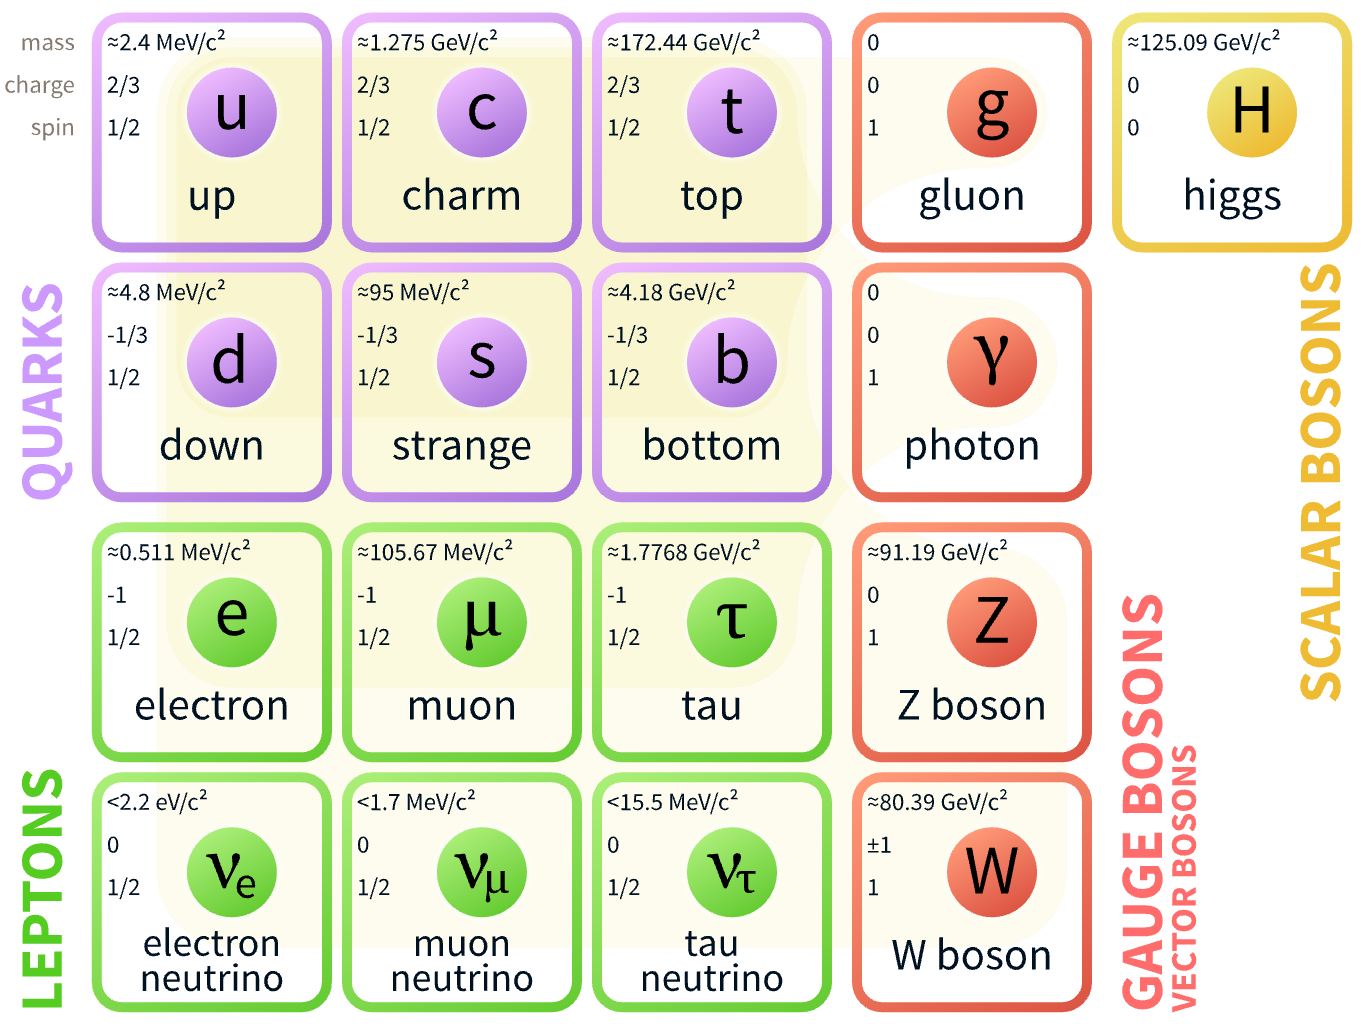
\includegraphics[width=0.6\textwidth]{figures/theory/SM}
  \caption{Fermions and bosons of the Standard Model and their properties~\cite{Pdg}, where all the values are measured experimentally.}
  \label{fig:SM}
\end{figure}

\paragraph{}
%However, in SM, due to the gauge invriance under $SU(2)_{L}$, fermions have to be massless in order to have pure left handed states. 
%The bosons must also be massless as required by the gauge principle. 
In the SM, the Higgs mechanism introduces a complex scalr Higgs field, $\phi$, with nonzero vaccum expectation values. Through spontaneous symmetry breaking of the Higgs potential $V(\phi) = -\nu^2\lambda_{\rm \nu} \phi^{\dagger}\phi + \lambda_{\rm \nu}(\phi^\dagger\phi)^2$, $W^{\pm}$ and $Z$ bosons aquire their masses. This process also predicts an extra scalar, the Higgs boson. The SM Lagrangian containing Higgs couplings, $\mathcal{L}_{\rm Higgs}$, is shown in Eq~\ref{eqn:higgspotential}.
\begin{equation}
\label{eqn:higgspotential}
% V(\phi_{h}) = \lambda \nu^2 \phi_{h} ^2  + \lambda \nu \phi_{h} ^3  + \frac{1}{4}\lambda \phi_{h} ^4 
\mathcal{L}_{\rm Higgs} = -g_{hf\bar{f}} hf\bar{f} + \delta_{V} V_{\rm\mu} V^{\rm\mu}\left(g_{\rm hVV} h + \frac{g_{\rm hhVV}}{2}h^2\right) + \frac{g_{\rm hh}}{2}h^2 + \frac{g_{\rm hhh}}{6}h^3 + \frac{g_{\rm hhhh}}{24}h^4 
\end{equation}
where 
\begin{itemize}
	\item $\rm\nu \sim 246$ \GeV, is the non-zero expectation value of the Higgs field;\
	\item $m_{\rm h} = \sqrt{2\lambda_{\rm \nu}}\nu \sim 125$ \GeV, is the Higgs mass; this is discovered in 2012\cite{ATLASHiggsDisc, CMSHiggsDisc}; 
	\item $\lambda_{\rm \nu}$, coefficient for the quartic potential term, is constrained from Higgs mass, to be $\sim 0.13$;
	\item $V = W^{\pm}$ or $Z$, $\delta_{W} = 1$, $\delta_{Z} = \frac{1}{2}$;
	\item $g_{hf\bar{f}} = \frac{m_{\rm f}}{\rm\nu}$, is the Higgs to fermion coupling; $m_{\rm f}$ is the mass of the fermion;
	\item $g_{\rm hVV} = \frac{2m_{\rm V}^2}{\rm\nu}$, is the Higgs to boson coupling; $m_{\rm V}$ is the mass of the boson;
	\item $g_{\rm hhVV} = \frac{2m_{\rm V}^2}{\rm\nu^2}$, is the Higgs-Higgs to boson-boson coupling;
	\item $g_{\rm hh} = m_{\rm h}^2$, is the Higgs mass term;
	\item $g_{\rm hhh} = \frac{3m_{\rm h}^2}{\rm\nu} = 6 \lambda_{\rm \nu} \nu$, or $\lambda_{\rm hhh}$, is the Higgs self-coupling;
	\item $g_{\rm hhh} = \frac{3m_{\rm h}^2}{\rm\rm\nu^2}$, is the Higgs quartic-coupling.
\end{itemize}
\paragraph{}
What's particularly interesting in Eq~\ref{eqn:higgspotential} is the $\frac{g_{\rm hhh}}{6}h^3$ term. This coefficient $\frac{g_{\rm hhh}}{6}$, or $\lambda_{\rm hhh}$, is also refered as \textbf{$\lambda_{\rm SM}$} in this thesis.
%A different coupling from $\lambda_{\rm SM}$ is usually refered as just $\lambda$. 
This term shows one way for two Higgs production with in the SM. Double Higgs production is also known as \textbf{di-Higgs or Higgs pair production}.

%Di-Higgs final states will provide complementary information from single Higgs physics at the LHC.
%Measuring this coefficient is one of the major tasks of experimental particlar physics program.

%%%%%%%%%%%%%%%%
\section{Standard Model di-Higgs production}

% \begin{figure}[h!]
%   \centering
%   \captionsetup{justification=centering}
%   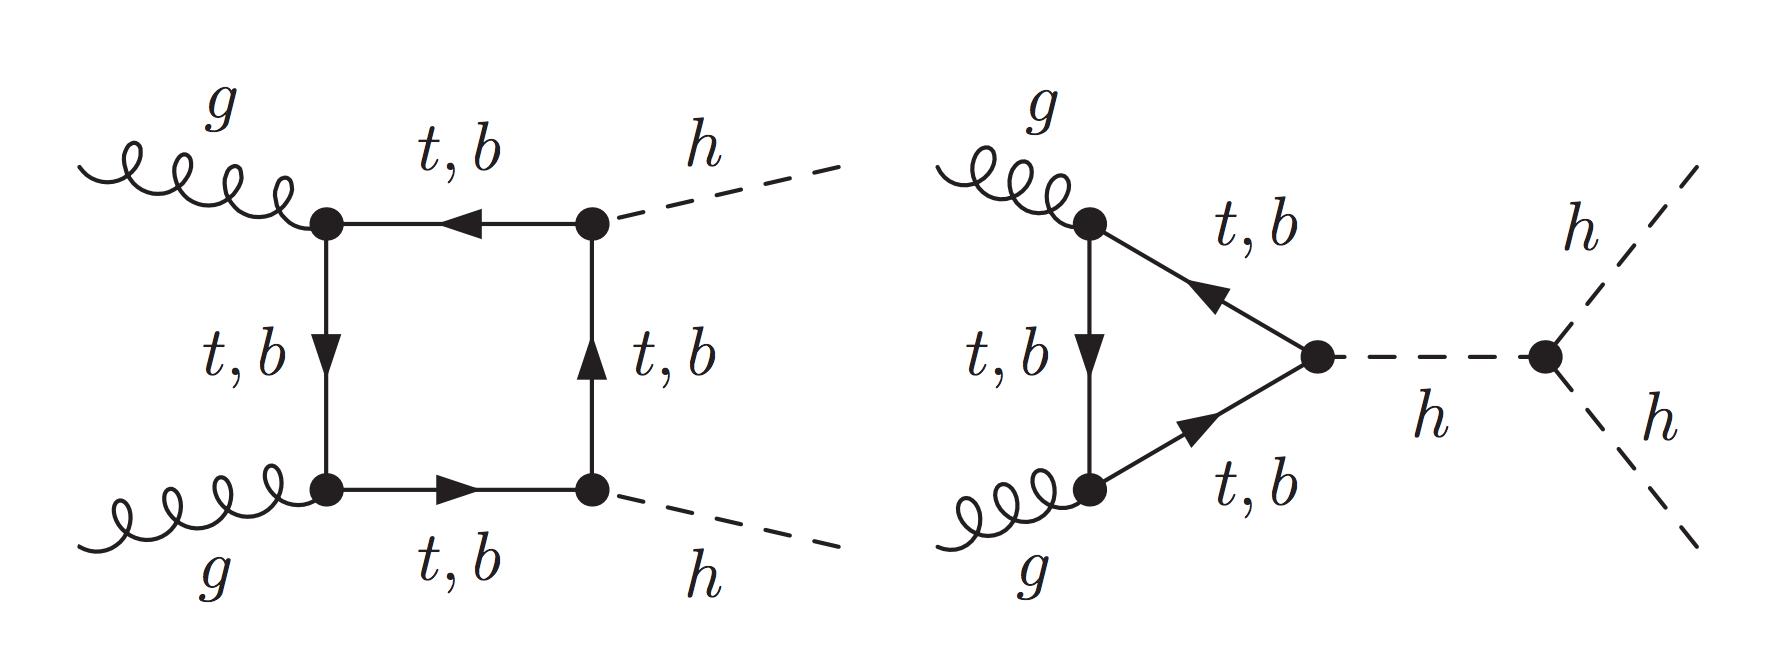
\includegraphics[width=0.7\textwidth]{figures/theory/SM_HH}
%   \caption{Feynman diagrams contributing to di-Higgs production via gluon-gluon fusion, through a $t$ or $b$ quark loop, at leading order. Only the right hand plot probes $\lambda_{hhh}$.}
%   \label{fig:SM_HH}
% \end{figure}

% \paragraph{}
% In the SM, the Higgs boson pair production through the $\lambda_{\rm hhh}$ has an on-shell component and a large off-shell component. The on-shell is strongly disfavored, requiring two off-shell Higgs bosons in the final state. The sensitivity region to the trilinear coupling production as in ~\ref{fig:SM_HH_tri}, is mainly in the kinematic region where the two Higgs boson in the final state are on-shell and the Higgs boson acts as a propagator (off-shell).

\paragraph{}
There are two main production mode of di-Higgs at the LHC, shown in Figure~\ref{fig:SM_HH}. In the gluon-gluon  fusion process, di-Higgs are produced through a box or a triangle loop (both mainly of top quarks). Only the triangle loop~\ref{fig:SM_HH_tri} probes the $\lambda_{hhh}$. This is showing the off-shell component, where the middle Higgs boson acts as a propagator (off-shell) and the two Higgs boson in the final state are on-shell. The on-shell component, with two off-shell Higgs bosons in the final state, is strongly disfavored~\cite{Pdg}. The two diagrams interfere distructively, which makes the overall production rate smaller than what would be expeced in the absence of a $\lambda_{hhh}$ term.

\begin{figure}[h!]
\centering
\captionsetup{justification=centering}
    \begin{subfigure}[b]{0.4\textwidth}
        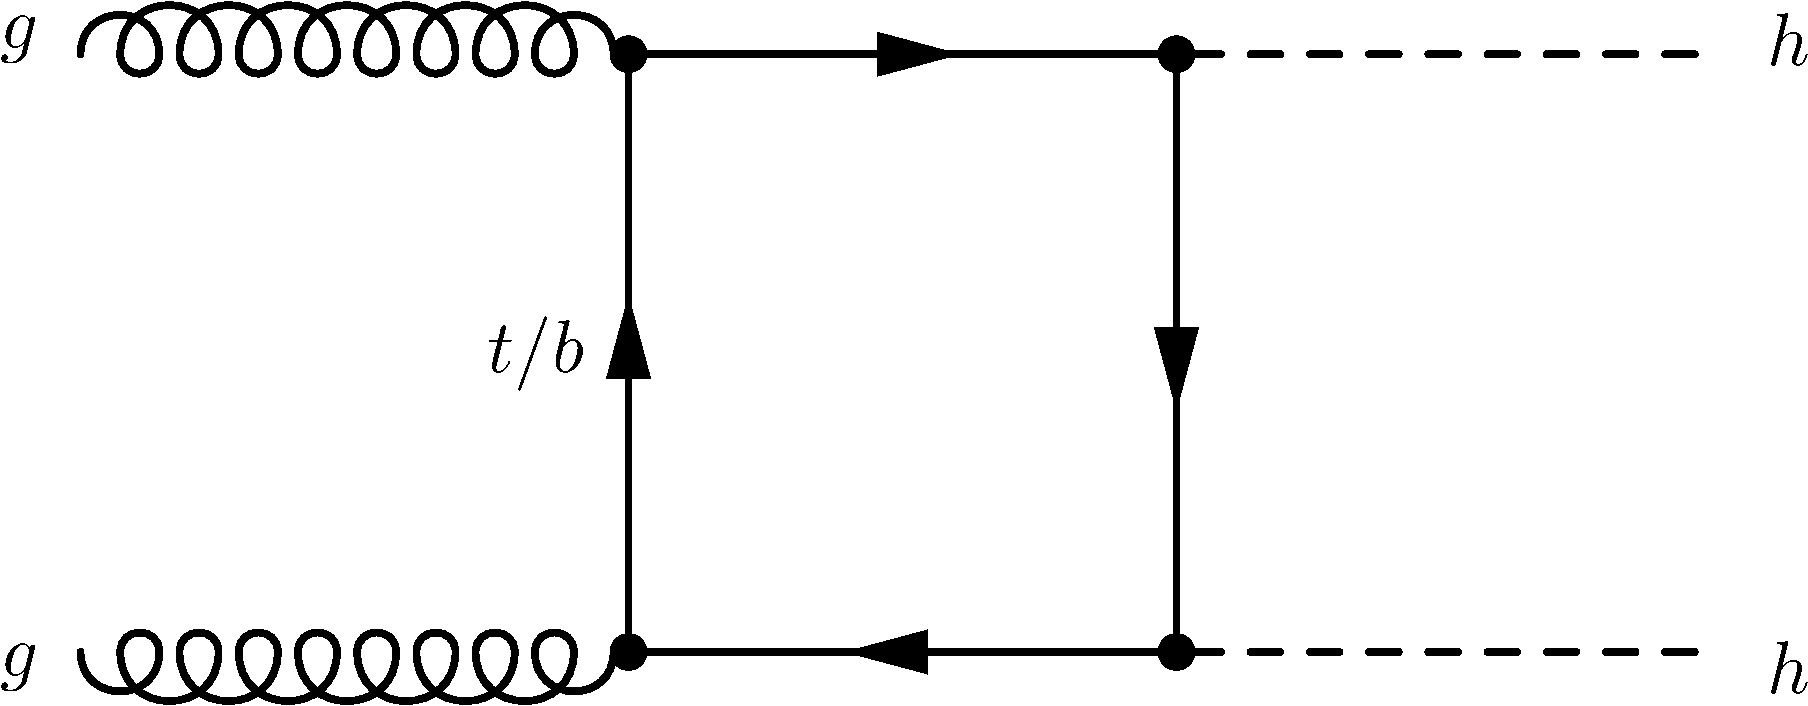
\includegraphics[width=\textwidth]{figures/theory/SM_HH_box}
        \caption{Box diagram}
        \label{fig:SM_HH_box}
    \end{subfigure}
    \quad
    \begin{subfigure}[b]{0.4\textwidth}
        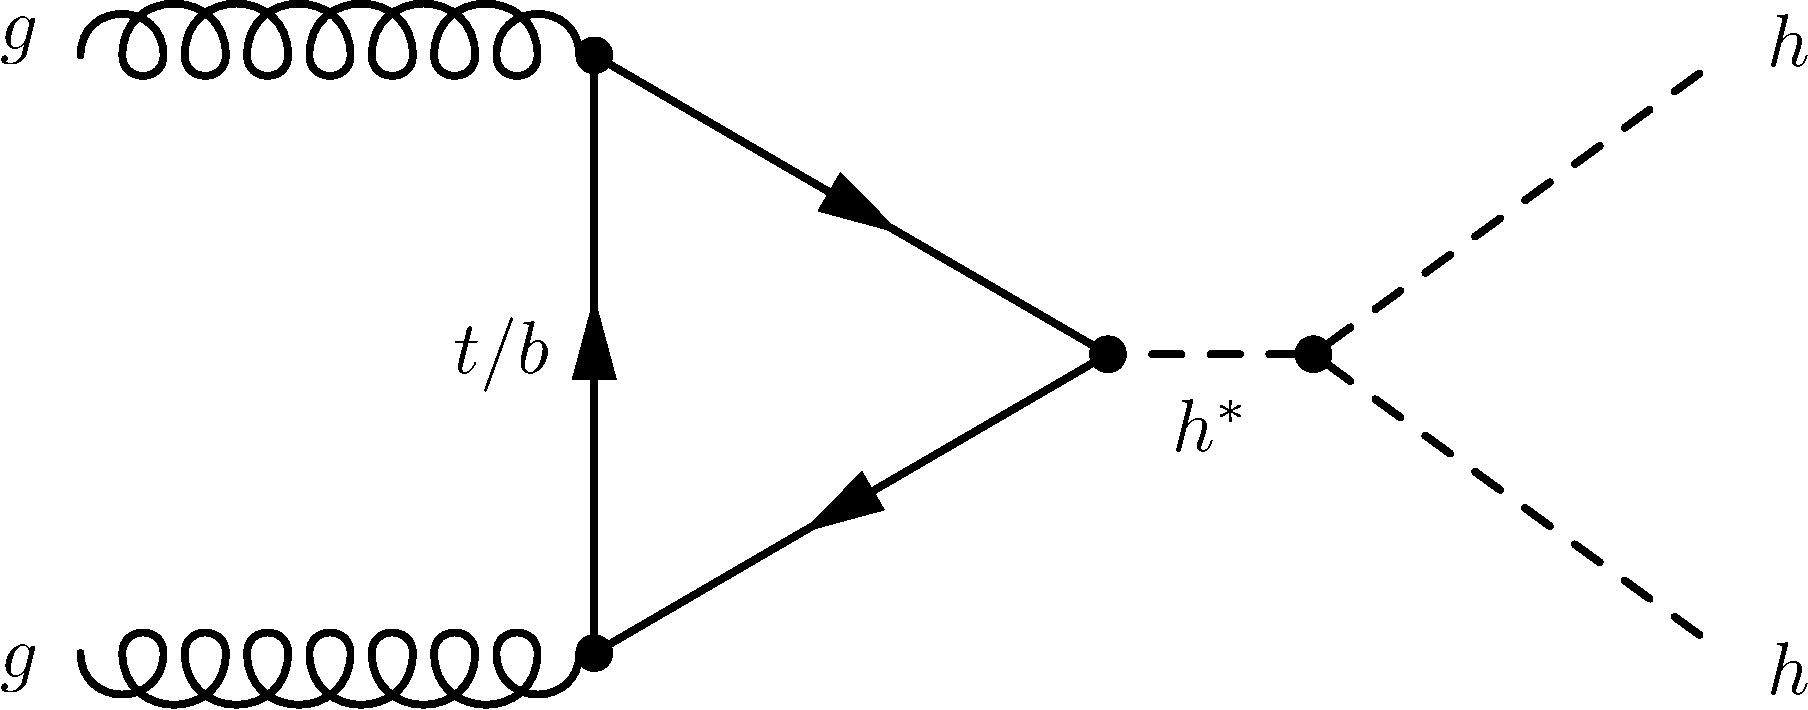
\includegraphics[width=\textwidth]{figures/theory/SM_HH_tri}
        \caption{Triangle diagram}
        \label{fig:SM_HH_tri}
    \end{subfigure}
\caption{Feynman diagrams contributing to di-Higgs production via gluon-gluon fusion, through the Higgs-fermion Yukawa interactions~\ref{fig:SM_HH_box} the Higgs boson self-coupling~\ref{fig:SM_HH_tri}, at leading order. Only Figure~\ref{fig:SM_HH_tri} probes $\lambda_{hhh}$.}
\label{fig:SM_HH}
\end{figure}

\paragraph{}
Many other different production modes of di-Higgs exists, but gluon-gluon fusion is the dominant one. Figure~\ref{fig:SM_HH_xsec}~\cite{Frederix:2014hta} compares gluon-gluon fusion, Vector Boson Fusion (VBF), and top-pair, $W^{\pm}$, $Z$ and single-top associated di-Higgs production.

\begin{figure}[h!]
  \centering
  \captionsetup{justification=centering}
  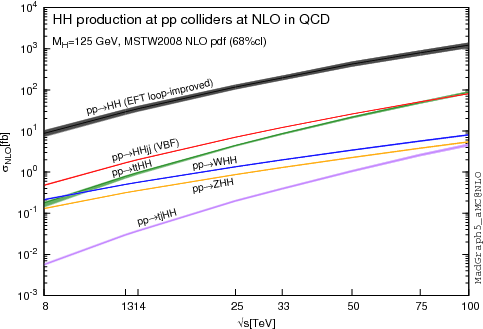
\includegraphics[width=0.7\textwidth]{figures/theory/HH_xsec}
  \caption{Total cross sections (y-axis) at the NLO in QCD for the six largest di-Higgs production channels at p-p colliders at different energy (x-axis). The thickness of the lines corresponds to the scale and PDF uncertainties added linearly. $H$ refers to the SM Higgs.}
  \label{fig:SM_HH_xsec}
\end{figure}

\paragraph{}
The total cross section for SM gluon fusion di-Higgs producion~\cite{LHCYellow}, at the Next to Next Leading Order (NNLO) with top quark mass effects, is $33.49^{+ 4.3 \%}_{-6.0 \%} \pm 2.1\% \pm 2.3\%$ fb for p-p collisions at $\sqrt{s}=13$ \TeV. The cross section for the next dominante production, VBF, is $1.62^{+ 2.3 \%}_{-2.7 \%} \pm 2.3\%$ fb. The eistiamted cross section for triple-Higgs production is $0.06332 ^{+ 16.1 \%}_{-14.1 \%} \pm 3.4\% $ fb, which is negeligiable. The uncertainties are Scale uncertainty, PDF uncertainty and $\alpha_s$ uncertainty. This means inside 2015 and 2016 $\sqrt{s}=13$ \TeV ATLAS data at 36 \ifb, there are only on the order of one thousand SM di-Higgs events.


%%%%%%%%%%%%%%%%
\section{Beyond the Standard Model Physics di-Higgs production}
\paragraph{}
BSM physics could significantly enhance the production of di-Higgs at the LHC. This is separated into two categories: non-resonant and resonant productions. The non-resonant production generally refers to modifications of the Higgs couplings, either the Higgs self-coupling or the Higgs-top couplings. Resonant production refers to a particle with invariant mass greater than twice the Higgs mass decays directly into two Higgs bosons. The difference also comes from the distribution of the di-Higgs invariant mass at the truth level. In the non-resonant case, the distribution has no clear peak, whereas in the resonant case, the invariant mass distribution forms a peak with model-depdent width.

\begin{figure}[h!]
\centering
\captionsetup{justification=centering}
    \begin{subfigure}[b]{0.3\textwidth}
        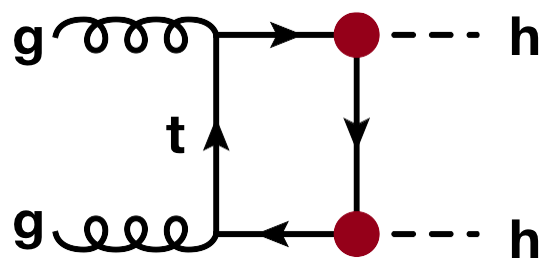
\includegraphics[width=\textwidth]{figures/theory/BSM_HH_box}
        \caption{$H$-fermion vertices variations}
        \label{fig:BSM_HH_box}
    \end{subfigure}
    \quad
    \begin{subfigure}[b]{0.3\textwidth}
        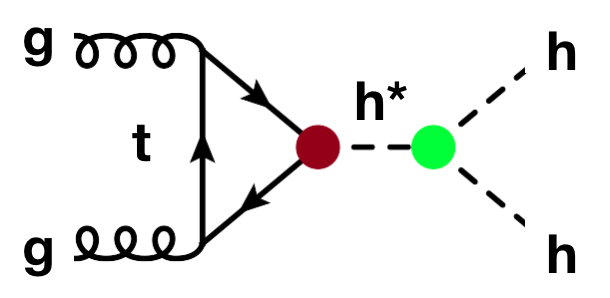
\includegraphics[width=\textwidth]{figures/theory/BSM_HH_tri}
        \caption{Higgs self-coupling variations}
        \label{fig:BSM_HH_tri}
    \end{subfigure}
    \quad
    \begin{subfigure}[b]{0.3\textwidth}
        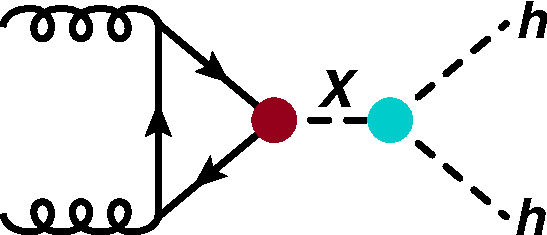
\includegraphics[width=\textwidth]{figures/theory/BSM_HH_X}
        \caption{an intermidiate resonance, X}
        \label{fig:BSM_HH_X}
    \end{subfigure}
\caption{BSM Higgs boson pair production: non-resonant production proceeds through changes in the SM Higgs couplings in~\ref{fig:BSM_HH_box} and~\ref{fig:BSM_HH_tri}, resonant production proceeds through~\ref{fig:BSM_HH_X} an intermediate resonance, X. $H$ and $h$ both refers to the SM Higgs.}
\label{fig:BSM_HH}
\end{figure}

\paragraph{}
Enhanced non-resonant Higgs boson pair production is predicted by many models. Models featuring direct $t\bar{t}\hh$ vertices \cite{Grober:2010yv, Contino:2012xk} or new light coloured scalars \cite{PhysRevD.86.095023} could change vertices shown as the red dots in Figure~\ref{fig:BSM_HH}. A direct modification of Higgs self-coupling term in Eq~\ref{eqn:higgspotential} to $\lambda hhh$, where $\lambda$ is different from $\lambda_{\rm sm}$, is also possible. This is shown as the green dot in Figure~\ref{fig:BSM_HH_tri}. The non-resonant di-Higgs enhancement is usually described by $\frac{\rm \lambda}{\rm \lambda_{\rm SM}}$, which is the cross section ratio between $\lambda$ and $\lambda_{\rm SM}$. Within the SM, from the electroweak measurements, the self coupling term could be constrained to $-14 \leq \frac{\rm \lambda}{\rm \lambda_{\rm SM}} \leq 17.4$~\cite{Kribs:2017znd}. Variations of $\lambda$ have a non-trivial effect on di-Higgs production cross section, shown in Figure~\ref{fig:SM_HH_lam}~\cite{Frederix:2014hta}.

\begin{figure}[h!]
  \centering
  \captionsetup{justification=centering}
  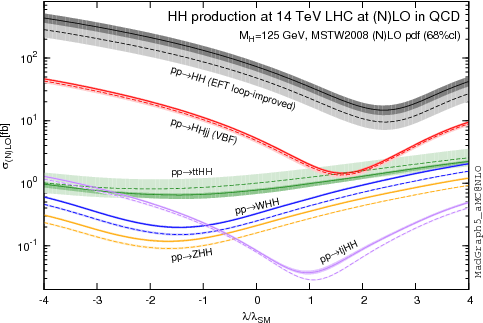
\includegraphics[width=0.7\textwidth]{figures/theory/HH_lam}
  \caption{Total cross sections (y-axis) at the LO and NLO in QCD for di-Higgs production channels, at the $\sqrt{s} = 14$ TeV LHC as a function of the self-interaction coupling $\lambda$ (x-axis) . The dashed (solid) lines and light- (dark-) colour bands correspond to the LO (NLO) results and to the scale and PDF uncertainties added linearly. The SM values of the cross sections are obtained at $\frac{\rm \lambda}{\rm \lambda_{\rm SM}} = 1$. $H$ refers to the SM Higgs.}
  \label{fig:SM_HH_lam}
\end{figure}

\paragraph{}
Resonant Higgs boson pair production is predicted by models such as the bulk Randall--Sundrum model~\cite{Agashe:2007zd,Fitzpatrick}, which features spin-2 Kaluza--Klein gravitons, \Grav, that subsequently decay to pairs of Higgs bosons. Extensions of the Higgs sector, such as two-Higgs-doublet models~\cite{PhysRevD.8.1226, Branco:2011iw}, propose the existence of a heavy spin-0 scalar that can decay into di-Higgs. 

\paragraph{}
The Randall-Sundrum model is a proposed solution to the hierarchy problem that posits a five-dimensional warped spacetime that contains two branes: one where the force of gravity is very strong and a second brane at the \TeV scale corresponding to the known Standard Model sector~\cite{RSG1}. In the theory, the branes are weakly coupled and the graviton probability function drops exponentially going from the gravity brane to the SM brane, rendering gravity weak on the SM brane. The experimental consequence of this theory is a tower of widely spaced (in mass) Kaluza-Klein graviton resonances. In theories where the fermions are localized to the SM brane, production of gravitons from fermion pairs is suppressed and the primary mode of production is gluon fusion~\cite{RSG_LHC}. These gravitons have a substantial branching fraction to Higgs pairs, ranging from $6.43$\% for gravitons with a mass of $500$ \GeV to $7.66\%$ at $3$ \TeV. Figure~\ref{fig:G_BR} shows the branching ratios of the spin-2 Randall Sundrum graviton (RSG) as a function of its mass. The predominant decays are to \ttbar above the mass threshold for that channel. 

\paragraph{}
Randall-Sundrum models have two free parameters - the mass of the graviton and a curvature parameter $k$. Typically, rather than $k$, the theory is parameterized using $c \equiv k/\bar{M}_{\rm pl}$, where $\bar{M}_{\rm pl}$ is the reduced Planck mass. The cross section for production of the RSG decreases as a function of mass and is strongly dependent on the gluon PDF. The increase in center of mass energy from $8$ to $13$ \TeV in LHC Run 2 greatly increases the cross section at higher mass. Figure~\ref{fig:G_xsec} shows the cross section as a function of graviton mass at $\sqrt{s} = 13$ \TeV for RSG models with $c=1.0$ and $c=2.0$. 

\paragraph{}
Another interesting feature of the theory is that the width of the graviton increases with both $c$ and mass. Figure~\ref{fig:G_width} shows the graviton width for both $c=1.0$ and $c=2.0$ as a function of mass. In $c=1.0$, the width starts at $8.365 \GeV$ for a mass of $300 \GeV$ and increases to $187.2 \GeV$ at a mass of $3 \TeV$. Similarly, with $c=2.0$, the width starts at $33.46 \GeV$ for $m_G = 300 \GeV$ and increases to $748.8 \GeV$ at a mass of $3 \TeV$. 

\paragraph{}
In Two Higgs Doublet Models (2HDM), a second complex scalar doublet is added to the Standard Model~\cite{HH_2HDM,2HDM2,2HDM3}. In this case, all four degrees of freedom in the second doublet correspond to new particles, meaning that there are five total scalars from the two Higgs doublets - $h$ (light CP-even Higgs), $H$ (heavy CP-even Higgs), $A$ (heavy CP-odd Higgs), and $H^{\pm}$ (charged Higgs). The model is parameterized by two main parameters. The first, $\tan{\beta} \equiv \frac{v_2}{v_1}$, is the ratio of the vacuum expectation values of the two Higgs doublets (where $v_1$ corresponds to the $v$ in the SM Higgs model described above). The second parameter is $\alpha$, a mixing angle between the heavy and light Higgs fields. Models are also often parameterized with $\cos(\beta - \alpha)$ rather than $\alpha$ directly. The limit where $\cos(\beta - \alpha) = 0$ is called the alignment limit, and in this limit the light Higgs $h$ has the same couplings as a Standard Model Higgs. Measurements of the Higgs boson have put constraints on these two parameters, but near the alignment limit there is still much unprobed phase space depending on the exact models and values of $\tan{\beta}$ being considered~\cite{HiggsNewPhysics}.

\paragraph{}
2HDM models are usually separated into two main types - Type I and Type II. In Type I models, the charged fermions only couple to the second Higgs doublet, leading to a fermiophobic light Higgs. In Type II models, up-type quarks couple to the first doublet while down-type quarks couple to the second doublet. One specific realization of a Type II 2HDM is the Minimal Supersymmetric Standard Model (MSSM).

\paragraph{}
Resonant di-Higgs production in 2HDM models can proceed through decays of the heavy CP-even Higgs $H\to hh$. The branching ratio for $H\to hh$ depends on the model type as well as the values of $\tan{\beta}$ and $\cos{\beta - \alpha}$. Figure~\ref{fig:H_BR} shows the branching ratios as a function of the mass of the heavy scalar $H$ for both Type I and Type II models. Depending on the type of model, $hh$ can be a substantial fraction of the decays of $H$. 

\paragraph{}
With the increased center of mass collison energy, the production cross section grows, particularly for heavy particles above TeV.


\section{Di-Higgs Decay}
\paragraph{}
Di-Higgs decay is the combination of single Higgs decays. 

%The partile width for Higgs to fermions and bosons (one of them is off-shell) at tree level are shown in equation~\ref{eqn:higgswidth}~\cite{Djouadi}:
% \begin{equation}
% \label{eqn:higgswidth}
% \begin{array}{cc}
% \Tau(h\to f\bar{f} ) = \frac{N_c \sqrt{2} G_{F} m_{f}^2 m_h}{8 \pi} \\
% \Tau(h\to VV^{*} ) = \frac{1}{\pi^2} \int_{0}^{M_H^2} \frac{dq_1^2 M_V \Gamma_V}{(q_1^2-M_V^2)^2 + M_V^2\Gamma_V^2} \int_0^{(M_H - q_1)^2} \frac{dq_2^2 M_V \Gamma_V}{(q_2^2-M_V^2)^2 + M_V^2\Gamma_V^2} \frac{\sqrt{2} \delta_v G_{F} m_h^3}{32\pi} \sqrt{\lambda(q_1^2, q_2^2; m_h^2)} [\lambda(q_1^2, q_2^2; m_h^2) + 12\frac{q_1^2q_2^2}{m_h^2}]
% %\Tau(h\to WW ) = \frac{2 \sqrt{2} G_{F} m_{W}^2 m_h}{32 \pi} \frac{\sqrt{1 - x_W}}{x_W^2} (3x_W^2 - 4x_w + 4) \\ %only for on shell
% %\Tau(h\to ZZ ) = \frac{\sqrt{2} G_{F} m_{z}^2 m_h}{32 \pi} \frac{\sqrt{1 - x_z}}{x_z^2} (3x_z^2 - 4x_z + 4)
% \end{array}
% \end{equation}
%where $N_c$ is the number os colors, $m_f$ is the fermion mass, $G_{F}$ is the Fermi constant. Hence, given the measured Higgs mass, tthe larges brancing ratio is to the \bbbar. Although there is no direct coupling between $h$ and \gg~ at tree level, this decay can happen through W or top loops.

\section{LHC previous search results}

\paragraph{}
Previous searches for Higgs boson pair production have all yielded null results. In the \bbbb~channel, ATLAS searched for both non-resonant and resonant production in the mass range of 400--3000~\GeV\ using 3.2 $\mathrm{fb}^{-1}$ of 13~\TeV\ data~\cite{EXOT-2015-11} collected during 2015. CMS searched for the production of resonances with masses of 750--3000~\GeV\ using 13~\TeV\ data~\cite{CMS-B2G-16-026} and with masses 270--1100~\GeV\ with 8~\TeV\ data~\cite{CMS-HIG-14-013}. Using 8~\TeV\ data, ATLAS has examined the \bbbb~\cite{Aad:2015uka}, \bbgg~\cite{HIGG-2013-29}, \bbtautau and \WWgg channels, all of which were combined in Ref.~\cite{HIGG-2013-33}. CMS has performed searches using 13~\TeV\ data for the \bbtautau~\cite{CMS-HIG-17-002} and $bb\ell\nu\ell\nu$~\cite{CMSHIG17006} final states, and used 8~\TeV\ data to search for \bbgg~\cite{Khachatryan:2016sey} in addition to a search in multilepton and multilepton+photons final states~\cite{Khachatryan:2014jya}.

%CMS latest search result on di-Higgs is also included \href{https://arxiv.org/pdf/1708.08249.pdf}{here}.